\documentclass{tufte-handout}

%\geometry{showframe}% for debugging purposes -- displays the margins

\usepackage{amsmath}


% Set up the images/graphics package
\usepackage{graphicx}
\setkeys{Gin}{width=\linewidth,totalheight=\textheight,keepaspectratio}
\graphicspath{{graphics/}}


% The following package makes prettier tables.  We're all about the bling!
\usepackage{booktabs}

% The units package provides nice, non-stacked fractions and better spacing
% for units.
\usepackage{units}

% The fancyvrb package lets us customize the formatting of verbatim
% environments.  We use a slightly smaller font.
\usepackage{fancyvrb}
\fvset{fontsize=\normalsize}

% Set up the spacing using fontspec features
\renewcommand\allcapsspacing[1]{{\addfontfeature{LetterSpace=15}#1}}
\renewcommand\smallcapsspacing[1]{{\addfontfeature{LetterSpace=10}#1}}

% Small sections of multiple columns
\usepackage{multicol}

% Provides paragraphs of dummy text
\usepackage{lipsum}

\usepackage{lettrine} % The lettrine is the first enlarged letter at the beginning of the text

% These commands are used to pretty-print LaTeX commands
\newcommand{\doccmd}[1]{\texttt{\textbackslash#1}}% command name -- adds backslash automatically
\newcommand{\docopt}[1]{\ensuremath{\langle}\textrm{\textit{#1}}\ensuremath{\rangle}}% optional command argument
\newcommand{\docarg}[1]{\textrm{\textit{#1}}}% (required) command argument
\newenvironment{docspec}{\begin{quote}\noindent}{\end{quote}}% command specification environment
\newcommand{\docenv}[1]{\textsf{#1}}% environment name
\newcommand{\docpkg}[1]{\texttt{#1}}% package name
\newcommand{\doccls}[1]{\texttt{#1}}% document class name
\newcommand{\docclsopt}[1]{\texttt{#1}}% document class option name


%%% Additions to template by DSL
\usepackage{hyperref} % provides \url{}
% remove separation between list items http://tex.stackexchange.com/a/10689/1783
\usepackage{enumitem}
\setlist{nosep}

% RMF additions
\usepackage{xcolor,colortbl}
\definecolor{green}{rgb}{0.1,0.1,0.1}
\newcommand{\grayout}{\cellcolor{lightgray}}
\newcommand{\hcyan}[1]{{\color{teal} #1}}

\usepackage{booktabs}

\usepackage{abraces}

\title{Emergence in Network Automata}
\author{Richard Foard}
\date{7 October 2018}  % if the \date{} command is left out, the current date will be used
\begin{document}

\maketitle% this prints the handout title, author, and date
\marginnote{\textsc{Contact:\\
Richard Foard\\
email: richard.foard@gtri.gatech.edu\\
phone: 404-281-3487
}}


\begin{abstract}
\noindent A simple, rule-based
graph automaton was defined and simulated. Each of its possible rules specifies a set
of local topology and node state changes to be applied iteratively, starting with a random initial graph.
Simulation runs were performed using many different rules, each run terminating when its graph
collapsed or cycled.
Evolving and terminal graph states were analyzed macroscopically, using
aggregate statistics, and microscopically, by inspecting graph structures.
Results were compared with those from simulations of a machine that
iterated by applying random, rather than rule-based, changes. We found that...
\end{abstract}

\section{Introduction}

\newthought{Since Alan Turing conceived his
universal machine} in 1936, simple abstract automata have drawn research attention.
Interest broadened beyond the academic realm in 1970,
when Conway published his \textit{Game of Life} simulations (citation needed) that highlighted the ability
of uncomplicated cellular automata to behave in complex ways. Researchers in the
nascent field of complexity theory began studying similar phenomena, such as the
sandpile avalanches first explored by Per Bak (true??).

In \textit{A New Kind of Science} (199?), Stephen Wolfram methodically analyzed
a variety of cellular automata types. He found particular inspiration in the
behavior of a one-dimensional machine running "Rule 110." Among his observations were... (list
irreducibility, etc.)

\begin{marginfigure}
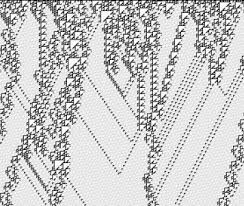
\includegraphics{rule110.jpeg}
\caption{Excerpt from the state sequence produced by Wolfram's \textit{Rule 110}
one-dimensional cellular automaton}
\end{marginfigure}

Wolfram and others have also suggested that some natural processes that were
previously thought to evolve by natural selection are instead
manifestations of things that nature found "easy" to accomplish using
the same fundamental principles that underlie simple automata.

In this work, we analyze simple graph automata using simulations of abstract
machines that operate on the same principles as
cellular automata but use a graph, rather than a "tape" or grid, as a substrate.
Where cellular machines define cell adjacency spatially, our machines use graph topology.


\section{Methods}

Two similar rule-based automata, \textbf{Machine C} and \textbf{Machine CM}, were designed
and implemented in simulation. The simulators were run repeatedly, using rules
selected at random from a large universe of possibilities. Measurements were recorded as the graphs
evolved through each run. The resulting database accumulated data on many thousands of runs. The body of data
was analyzed macroscopically, using aggregate statistics, and microscopically, by inspecting
statistical and graphic snapshots from individual runs.

\begin{marginfigure}
\hspace{-4em}
\includegraphics{5iters_0.ps}
\end{marginfigure}

\begin{marginfigure}
\hspace{-4em}
\includegraphics{5iters_1.ps}
\end{marginfigure}

\begin{marginfigure}
\hspace{-4em}
\includegraphics{5iters_2.ps}
\end{marginfigure}

\begin{marginfigure}
\hspace{-4em}
\includegraphics{5iters_3.ps}
\caption{Three iterations of machine \textbf{C}, rule 177828939654904,
beginning with a randomly generated 8-node graph and terminating in a
static configuration.}
\end{marginfigure}

Each simulation run begins with a randomly generated graph and progresses by
iteratively modifying its edges and node states; changes are made according to a rule selected
for the run. Each rule is effectively a simple program  that specifies, based on the state
of each node and its two topological neighbors, how local changes should be applied during an
iteration.

\subsection{Graph Composition}

Nodes may be in one of two states: \textit{black} or \textit{white}.
Graph topology is restricted in order to simplify rule design. For the
\textbf{CM} machine:

\vspace{1mm}
\begin{itemize}
\setlength{\itemindent}{2em}
    \item Edges are directed.
    \item Nodes have out-degree of exactly two.
    \item "Self-linking" edges are permitted.
\end{itemize}
\vspace{2mm}
The \textbf{C}  machine's graphs are more narrowly defined by adding the
restriction:
\begin{itemize} 
\setlength{\itemindent}{2em}
    \item Multiple, like-directed edges between two nodes are prohibited.
\end{itemize}
\vspace{2mm}

\textbf{C} and \textbf{CM} machines operate using the same rule structures.
A single rule is chosen for each run. Each execution
begins on a graph that has been randomly generated
to conform to its machine's topological restrictions. Both machines maintain conformance
throughout the run. In applying some rules, \textbf{C} creates prohibited
structures. When this occurs, a "pruning" process selectively
removes nodes and edges to restore conformance before proceeding with the
next iteration. The \textbf{CM} machine does not need this process because
it is structurally incapable of altering its graph in a way thati violates its more
relaxed structure restrictions. \textbf{CM} is otherwise identical to \textbf{C}.  

An initial, random graph of size N is constructed by assigning each node
a \textit{black} or \textit{white} state with equal likelihood.
Two edges are attached to each node, with
the destination of each selected at random from all nodes. For \textbf{C} runs, the
generator observes the constraint that both edges cannot have the same destination node.
In all initial graphs, nodes have out-degree 2, but in-degree can vary from 0 to N.
Initial graphs are a subset of the class of Erdos-Renyi random graphs (citation needed)
\textit{G(n, p)} where \textit{n} is the number of nodes and \textit{p} is the probability
that two nodes are connected by an edge. Because all graphs have fixed out-degree 2,
the generation process creates random variation only in the nodes' in-degrees. As a result,
each initial graph is a member of \textit{G(n, p)} where \textit{p} is a function
of graph size \textit{n} (approximately \( 4 / (n - 1) \)).

\subsection{Rule Structure and Application}

At the start of each simulation run, a rule is selected and an initial graph
is generated.  The simulation proceeds in a series of
iterations. During each, the rule is applied at each node, yielding a draft
version of a new graph. For machine \textbf{CM}, the draft immediately becomes
the input to the next iteration. In \textbf{C}, the draft may require pruning
before becoming input to the next iteration. 

During an iteration, each node in the current graph is examined in turn.
The combined \textit{black}/\textit{white} states of the node and its two neighbors\footnote{
\textit{Black} is interpreted as zero, \textit{white} as one. In
all cases, "neighbor" is used to indicate a node at the destination end of one of a node's out-edges.}
are used to select one of the rule's eight constituent parts; the selected part, in turn,
controls the changes that are made to the node's state and its out-edges in
the developing draft copy. Rules encode change instructions as follows:

A rule comprises eight parts, each corresponding to one of the possible compound, or "triad" states
of a node and its neighbors. Each rule-part specifies replacement values for
the node's state and the destinations of its out-edges
(it is convenient to refer to a node's two out-edges as "left" and "right").
The replacement node state is either \textit{black} (\textit{B}) or \textit{white} (\textit{W}).
The replacement edge destinations (Figure \ref{fig:Sixlabeled}) are each one of:

\vspace{1mm}
\begin{itemize}
\setlength{\itemindent}{2em}
    \item \textit{L} - the node's current left-edge destination
    \item \textit{R} - the node's current right-edge destination
    \item \textit{LL} - the current destination of its left neighbor's left-edge
    \item \textit{LR} - the current destination of its left neighbor's right-edge
    \item \textit{RL} - the current destination of its right neighbor's left-edge
    \item \textit{RR} - the current destination of its right neighbor's right-edge
\end{itemize}
\vspace{2mm}
A rule might be represented symbolically, for example, as:
\[
\aunderbrace[l1r]{L,L,B}_{0}; \aunderbrace[l1r]{R,RR,W}_{1}; \aunderbrace[l1r]{L,R,W}_{2}; \aunderbrace[l1r]{LL,R,B}_{3}; \aunderbrace[l1r]{L,LL,B}_{4}; \aunderbrace[l1r]{RL,RR,W}_{5}; \aunderbrace[l1r]{RR,RR,B}_{6}; \aunderbrace[l1r]{R,L,B}_{7}
\]
in which each semicolon-separated substring is a rule-part to be applied at nodes having a
triad state equal to the part's index position in the rule string. For coding purposes, rule
numbers are encoded as a mixed-radix integer between 0 and
$(6 \times 6 \times 2)^8 \quad (722,204,136,308,736)$.

\begin{marginfigure}
\hspace{-4em}
\includegraphics{sixlabeled.ps}
\caption{The six possible new destinations for node \textbf{*}'s out-edges}
\label{fig:Sixlabeled}
\end{marginfigure}

\vspace{1mm}
After all nodes in the original graph have been processed,
the resulting draft copy is pruned if necessary.
Applicable only for machine \textbf{C}, the pruning step removes
any like-directed edges (multi-edges) that have been created between pairs
of nodes in the draft copy; the process selectively removes nodes
and redirects edges, cascading as required, until no prohibited structures remain.
If it is not empty, the pruned graph becomes the starting point for the next iteration;
if it is empty, it is said to have collapsed.
A simulation run ends when (1) the graph collapses, (2) a state cycle is detected,
or (3) a maximum number of iterations is reached.

\subsection{The \textbf{C*} Machines' Random Counterparts, \textbf{R} and \textbf{RM}}

To help gauge the extent to which machines \textbf{C} and \textbf{CM}
introduce order as they transform random starting graphs, simulators for counterpart
machines \textbf{R} and \textbf{RM} were constructed. Like the rule-based \textbf{C*} machines,
these change the graph iteratively, but make their changes \textit{randomly}.
As with the \textbf{C*} machines, though, the scope of edge destination changes for each node is
limited to nodes reachable in its "two-hop" neighborhood. (The random machines need not alter nodes' states
because node states have no effect on the \textbf{R*} machines' actions).
The \textbf{R} machine applies the same pruning process that \textbf{C} uses. As
with \textbf{CM}, no pruning step is required in \textbf{RM} simulations because
no prohibited structures can be generated by the \textbf{*M} machines.

\begin{table}
\caption{Machine Characteristics}
\centering
\begin{tabular}{lccc}
\toprule
Machine & New Edge Selection & Multi-edges & Pruning Performed \\
\midrule
\textbf{C} & \textit{Rule-based} & \textit{No} & \textit{Yes} \\
\textbf{R} & \textit{Locally Random} & \textit{No} & \textit{Yes} \\
\cmidrule(r){2-4}
\textbf{CM} & \textit{Rule-based} & \textit{Yes} & \textit{No} \\
\textbf{RM} & \textit{Locally Random} & \textit{Yes} & \textit{No} \\
\bottomrule
\end{tabular}
\label{tab:Tab1}
\end{table}
\vspace{3mm}

\subsection{Graph Pruning}

Changes to out-edge destinations, whether made randomly by machine \textbf{R} or based on \textbf{C}'s
rules, can introduce multi-edges. These prohibited structures
arise as the machine's iteration logic creates a first-pass, "draft" copy of the transformed graph.
the draft copy is pruned to restore conformance with structure restrictions before
the following iteration begins.
The diagram in Figure \ref{fig:Pruning} shows the two kinds of prohibited structures
that can occur and illustrates the restorative changes made in the pruning step.

\begin{figure}
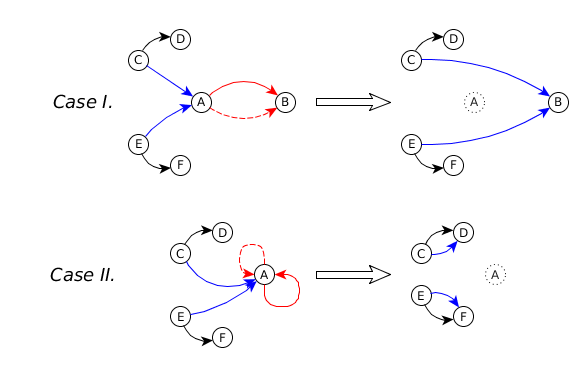
\includegraphics{pruning.png}
\caption{\textbf{Pruning.} Resolution methods for two variations of a (red) prohibited structure.
In both cases, edges originating at node A are eliminated; edges in blue are redirected.
Case II creates two case I-type structures that require further resolution.}
\label{fig:Pruning}
\end{figure}

Both types of changes eliminate the node at which the offending edge pair
originates (labeled "A" in the illustrations), along with the edge pair.
In case I, all edges inbound to the eliminated node are redirected to 
the destination (shown as node "B") of its to-be-eliminated edge pair.
Redirected edges are shown in blue.

Lacking such a natural new destination for the inbound edges in case II, the
pruning process instead moves the problem "upstream"---any edge inbound to
the eliminated node is redirected to the same destination node as that of
its origin node's other out-edge. This, of course, immediately creates
case I structure violations for all such origin nodes; these violations must also be
resolved before the next iteration can begin.
Case II resolutions \textit{always} create additional structure violations;
case I resolutions may or may not. In either case, cascades can result. These
cascades, and the resulting reductions in graph size, are common in both
\textbf{C} and \textbf{R} simulations.

\subsection{The Simulator}

Input parameters and statistics gathered. Data base and analysis tooling.
Constituent packages. How parameter values were selected and varied.

%------------------------------------------------

\section{Results}

In this section, a largely qualitative summary of simulation results is followed
by sections on the more interesting aspects of outcomes.

\subsection{Summary of Outcomes---Cycles and Collapses}

Each simulation run begins with a finite graph, and each iteration
either maintains the number of nodes or, in the cases of \textbf{C} and \textbf{R},
reduces it by pruning.  It is consequently certain that the machines always terminate,
either in a state cycle or in a graph collapse; this holds true
for all types: \textbf{C}, \textbf{CM}, and their random counterparts \textbf{R} and \textbf{RM}.
The possibility that a graph will traverse an astronomical number
of states\footnote{The number of possible states for an N-node graph with
out-degree restricted to 2 is:
\[
2^N\cdot\binom{N}{2}^N
\]
}
before revisiting a previous one, however, limits the simulator's ability to
detect cycles. If the simulator reaches a maximum number of iterations
before its machine terminates, the simulation outcome is recorded as "undetermined."
A summary of outcomes for all runs is given in Table \ref{tab:Tab2}.

\begin{table}
\caption{Simulation Outcomes, All Runs}
\centering
\begin{tabular}{lrcr}
\toprule
Machine & Cycling & Collapsed & Undet. \\
\midrule
\textbf{C} & 40.77\% & 59.22\% & 0.01\% \\
\textbf{R} & 0.01\% & 99.99\% & 0\% \\
\cmidrule(r){2-4}
\textbf{CM} & 99.07\% & --- & 0.03\% \\
\textbf{RM} & 100.00\% & --- & 0.00\% \\
\bottomrule
\end{tabular}
\label{tab:Tab2}
\end{table}
\vspace{3mm}

The reason that nearly all \textbf{CM} and \textbf{RM} runs end in state cycles is
intuitive---because they allow multi-edges, they tend to generate structures
like those in Figure \ref{fig:Multiedges}. These are virtually certain to appear
under \textbf{R}'s random edge reassignments, and highly likely for most of
\textbf{CM}'s rules. As these structures enter the graph, they 
shrink the number of possible new out-edge destinations for their origin nodes,
progressively decreasing the number of possible new states in the graph overall.

\begin{marginfigure}
%\hspace{-10mm}
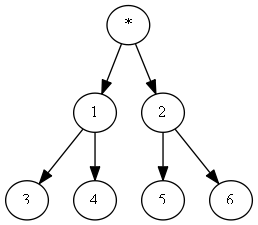
\includegraphics[scale=0.3]{sixchoices.png}
\caption{For each edge originating at the "*" node, there are six possible new destinations. (These
are not necessarily six different nodes, but are more likely to be distinct nodes when
multi-edges are not present.)}
\label{fig:Sixnumbered}
\end{marginfigure}

\begin{marginfigure}
\vspace{2mm}
\includegraphics{multiedges.ps}
\caption{Structures with multi-edges reduce the number of possible new edge destinations for
the origin ("*") node during each machine iteration.}
\label{fig:Multiedges}
\end{marginfigure}

The prohibition of multi-edges in machines \textbf{C} and \textbf{R}
necessitates the removal of prohibited structures when they arise. The
number of nodes in the graph can consequently decrease during execution,
often to the point of complete collapse.
Machine \textbf{R} is far more likely to produce graph collapses than
\textbf{C} is (99.9\% vs. 59.2\% of runs). The reason is similar to the reason
that \textbf{*M} machine runs collapse: just as \textbf{RM} produces multi-edges,
random variation will ensure that \textbf{R}'s same edge rerouting logic
will produce some number of structures that must be pruned out.
\textbf{C}, on the other hand, is more or less likely
to produce prohibited structures, depending on the rule in force for each particular
run.

In runs in which \textbf{C} produces
collapses, average run length is consistently greater than
for \textbf{R} (Figure \ref{fig:figA}), suggesting that
rule-based graph evolution, on average, produces prohibited structures
at a slower pace.

(Move this later) For both machine types, we refer to
the number of nodes at the end of the iteration immediately preceding a collapse,
or to the "settled" number of nodes in a cycling graph, as the terminal number of nodes.

<Compare cycling behaviors. ?Cycle lengths vs nr iterations?>

<Explain why further investigation of the *M machines was dropped.>

<Explain why R collapses are far more likely.>

<Discuss collapse shapes, R vs C.>

\begin{marginfigure}
  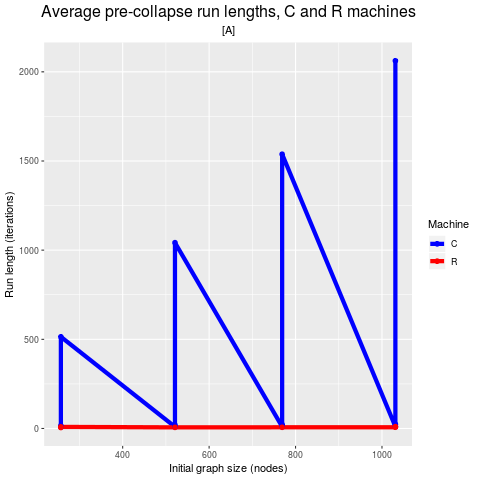
\includegraphics{figA.png}
  \caption{On average, the rule-based \textbf{C} machine executes more iterations than \textbf{R} before collapse occurs.}
  \label{fig:figA}
\end{marginfigure}

\subsection{In-Degree Entropy}

Machine \textbf{C}, on average, generates graphs with a larger 
maximum in-degree than in the random case of machine \textbf{R}, and also produces a
larger number of distinct in-degrees (Figure \ref{fig:figB}).

\begin{marginfigure}
  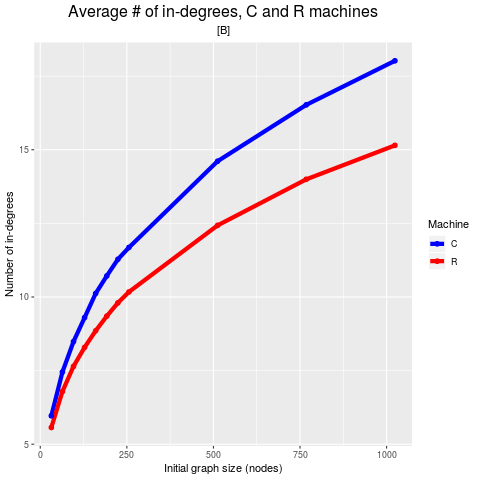
\includegraphics{figB.png}
  \caption{\textbf{C} produces graphs with a larger number of in-degrees.}
  \label{fig:figB}
\end{marginfigure}

Shannon's entropy [citation needed], computed on summary in-degree statistics and
normalized\footnote{Explanation of normalization}, can be regarded a measure of
a graph's "randomness."
As would be expected, entropy is consistently large in the randomly generated
initial graphs. Between the \textbf{R} and \textbf{C} machines, entropy in the terminal
graphs for \textbf{C} is lower than that for the randomly operating R (Figure \ref{fig:figE}).

The drop in average entropy between initial graphs and the \textbf{R} machine's terminal
graphs seems surprising on its face, but is accounted for by the restriction that
\textbf{R}'s topological changes, like \textbf{C}'s, may only redirect a node's out-edge
within its two-hop neighborhood.
The effect is to "localize" the randomness, abruptly increasing apparent order in the
random graph as soon as the first iteration is finished.

The two \textbf{*M} machines that allow multi-edges to remain in the graph, \textbf{CM} and
\textbf{RM}, almost invariably cycle because there are fewer possible new destinations for
both members of a multi-edge when the machine applies the iteration rule (or random choice
in the case of \textbf{RM}) at their origin node. <Refer to the diagram, then go on to
explain that the effect is more pronounced for the random variant because...>

\begin{marginfigure}
  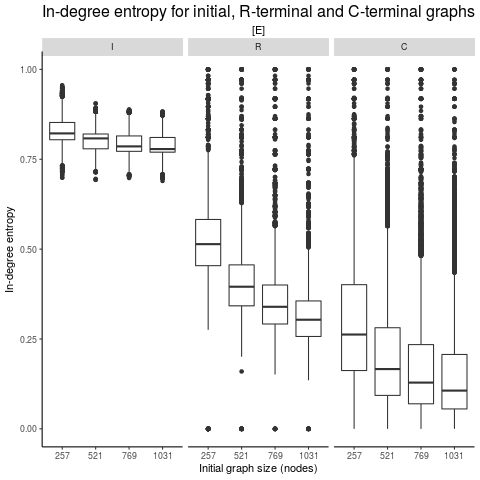
\includegraphics{figE.png}
  \caption{In-degree entropy is largest in initial random graphs,
        smaller for \textbf{R}'s terminal graphs, and smallest for \textbf{C}'s terminal graphs.}
  \label{fig:figE}
\end{marginfigure}

\begin{marginfigure}
  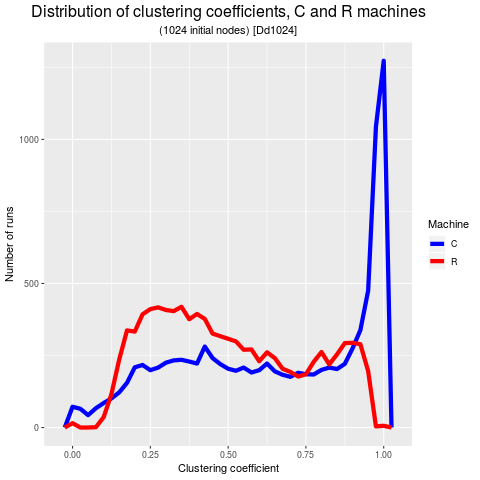
\includegraphics{figDd1024.png}
  \caption{\textbf{C}'s average clustering coefficients are larger than \textbf{R}'s.}
  \label{fig:figDd1024}
\end{marginfigure}

\subsection{Sensitivity to Initial Conditions}

<Discuss.>

\subsection{Degree Distribution}

\subsection{Clustering}

Terminal clustering coefficients for machine \textbf{C} are smaller than those for \textbf{R} in
the large majority of cases (Figure \ref{fig:figDd1024}).

This is where things get more interesting.

For this one, we'll have to dust off the old self-organizing criticality
references. Are collapses like sandpile avalanches?

\clearpage

\begin{table}
\caption{Table \ref{tab:TabQ}: Comparison of Graph Measures Across (Machine $\times$ Outcome)}
\vspace{12mm}
\centering
\begin{tabular}{lcccccccc}\toprule
\addlinespace[3mm]
Machine:  & \multicolumn{2}{c}{\textbf{C}} & \multicolumn{2}{c}{\textbf{CM}} & \multicolumn{2}{c}{\textbf{R}} \\ \midrule
\addlinespace[2mm]

Outcome: & \textit{Cycling} & \textit{Collapsed} & \textit{Cycling} & \textit{Collapsed} & \textit{Cycling} & \textit{Collapsed} \\ \cmidrule(lr){2-2} \cmidrule(lr){3-3} \cmidrule(lr){4-4} \cmidrule(lr){5-5} \cmidrule(lr){6-6} \cmidrule(lr){7-7}
\# Connected &  &  & \includegraphics[width=3cm, height=10cm]{rel_lo.png} & \grayout & \grayout & \\
Components & $\approx$ 1 & $\approx$ 1 & & \grayout & \grayout & $\approx$ 1  \\
  &  &  &  & \grayout & \grayout & \\
\addlinespace[2mm]

  &  &  &  & \grayout & \grayout & \\
\# Iterations & $\approx$ 1 & $\approx$ 1 & & \grayout & \grayout & $\approx$ 1  \\
  &  &  &  & \grayout & \grayout & \\
\addlinespace[2mm]

\# Terminal &  &  & highest & \grayout & \grayout & \\
Components & $\approx$ 1 & $\approx$ 1 & & \grayout & \grayout & $\approx$ 1  \\
  &  &  &  & \grayout & \grayout & \\ \bottomrule
\end{tabular}
\label{tab:TabQ}
\end{table}
\vspace{3mm}

\subsection{Designed Rules}
%Made to Order?
%Learning the Hard Way?
%Designer Rules? Rules by Design?

\subsection{Interesting Configurations}
%Photo Opps?
Sorter?

%------------------------------------------------

\section{Discussion}

Possible areas for further investigation:

\begin{itemize}
    \item Search strategies for rules with specific characteristics.
    \item Encodings of more complex graph structures.
    \item Exploring mathematical parallels.
    \item Investigating variations on the machines, both simpler and more complex.
\end{itemize}

A statement requiring citation \cite{Figueredo:2009dg}.

%----------------------------------------------------------------------------------------
%	REFERENCE LIST
%----------------------------------------------------------------------------------------

\begin{thebibliography}{99} % Bibliography - this is intentionally simple in this template

\bibitem[Figueredo and Wolf, 2009]{Figueredo:2009dg}
Figueredo, A.~J. and Wolf, P. S.~A. (2009).
\newblock Assortative pairing and life history strategy - a cross-cultural
  study.
\newblock {\em Human Nature}, 20:317--330.
 
\end{thebibliography}

\vspace{1cm}

\emph{This handout was based on an article I originally wrote for the Carolinia Farm Stewardship newsletter, March-April 2004.}

\end{document}
